\section{Experiments}
\label{sec:experiments}

\begin{figure}
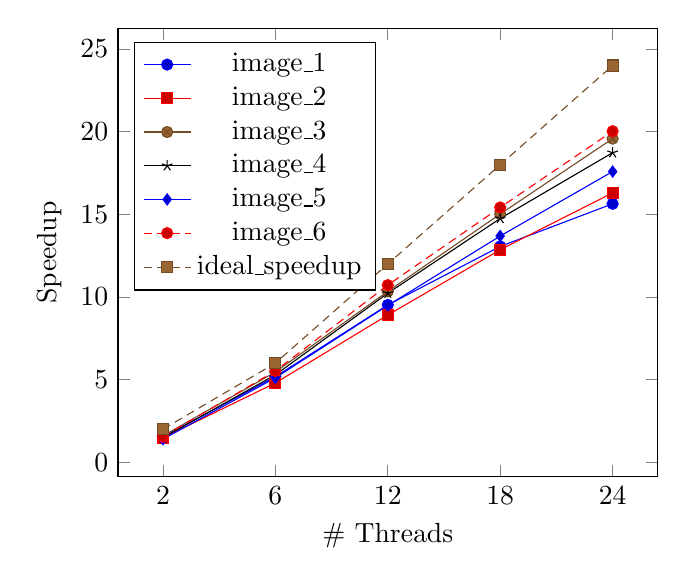
\begin{tikzpicture}
\begin{axis}[legend pos = north west,
xlabel=\# Threads,
ylabel=Speedup,
symbolic x coords={2,6,12,18,24}]
\addplot+[sharp plot] coordinates {
(2,1.54)
(6,5.18)
(12,9.52)
(18,13.06)
(24,15.64)
};
\addplot+[sharp plot] coordinates{
(2,1.48)
(6,4.80)
(12,8.91)
(18,12.86)
(24,16.30)
};
\addplot+[sharp plot] coordinates{
(2,1.60)
(6,5.46)
(12,10.34)
(18,15.02)
(24,19.58)
};
\addplot+[sharp plot] coordinates{
(2,1.49)
(6,5.29)
(12,10.23)
(18,14.75)
(24,18.73)
};
\addplot+[sharp plot] coordinates{
(2,1.40)
(6,5.11)
(12,9.49)
(18,13.69)
(24,17.59)
};
\addplot+[sharp plot] coordinates{
(2,1.55)
(6,5.53)
(12,10.72)
(18,15.42)
(24,20.03)
};
\addplot+[sharp plot] coordinates{
(2,2)
(6,6)
(12,12)
(18,18)
(24,24)
};
\legend{image\_1,image\_2,image\_3,image\_4,image\_5,image\_6,ideal\_speedup}
\end{axis}
\end{tikzpicture}
\caption{Speedup for different images and different numbers of threads for local + merge}
\label{linet}
\end{figure}


For the experiments we used Hopper. Hopper is NERSC's first peta-flop system, a
Cray XE6, with a peak performance of $1.28$ Petaflops/sec, $153,216$ compute
cores for running scientific applications, $217$ terabytes of memory, and $2$
petabytes of online disk storage. All algorithms were implemented in C using OpenMP and compiled with gcc.

Our test dataset consists of $4$ types of image dataset: Texture, Arial,
Miscellaneous and NLCD. First three datasets are taken from the image database of the University of 
Southern California\cite{}. The fourth dataset is taken from US National Cover Database
$2006$ \cite{}. All of the images are converted to binary images by means of MATLAB.
Texture, Arial and Miscellaneous dataset contain images of size $1024 \times
1024$ or less.
NCLD dataset contains images of size bigger than $3000 \times
4000$. The biggest image in the dataset is $22,822 \times 20,384$.

Firstly, we did the experiment over all the sequential algorithms. The
experimental results are shown in Table \ref{table:seq}. In the table, we have
shown the minimum, maximum and average execution time of all the $4$ datasets. 
\begin{table}[h]
\caption{Comparison of various execution times[{\em msec}] for sequential algorithms}
\centering
\begin{tabular}{c c c c c c} 
\hline\hline
Image type &  & CCLLRPC & CCLRemSP & ARun & ARemSP\\ [0.5ex] 
\hline 
Aerial & Min & 2.5 & 2.48 & 1.98 & 1.95 \\ 
 & Average & 13.68 & 13.25 & 11.90 & 11.86\\
 & Max & 86.64 & 80.90 & 72.92 & 70.17 \\
[1ex]
 \hline
Texture & Min &2.07 & 2.06 & 1.58 & 1.53 \\
 & Average & 8.42 & 8.20 & 7.32 & 7.27 \\
 & Max & 16.86 & 16.18 & 14.81 & 14.47\\
[1ex]
 \hline
Miscellaneous & Min & 0.50 & 0.49 & 0.36 & 0.36\\
 & Average & 3.28 & 3.21 & 2.75 & 2.74 \\
 & Max &12.96 & 12.81 & 11.30 & 11.20\\
 [1ex]
\hline
NLCD & Min & 4.61 & 4.46	& 3.77 & 3.75 \\
& Average & 307.66 & 299.55 & 244.88 & 242.59 \\
& Max & 1307.27	& 1273.82 & 1036.52 & 1021.45
\\[1ex]
\hline
\end{tabular}
\label{table:seq} 
\end{table}

As we can see that execution time of {\em ARemSP} is lowest among all
the sequential algorithms thus {\em ARemSP} is best among all the sequential
algorithms.
Then we tested the parallel algorithm {\em PARemSP} over all the images.
Fig \ref{line}-\ref{linet} shows the speedup of the algorithm for 
NCLD image dataset.The images are labeled in the increasing order of their
sizes. We get a maximum speedup of $20.1$ for image of size $22822 \times 20384$.
Fig \ref{line} shows the speedup for {\em Phase-$I$} of \paremsp\ i.e. 
the local computation and fig \ref{linet} shows the overall speedup (i.e. local + merge). We can see that there is not 
significant difference between both the speedups, implying that merge operation
does not have a significant overhead. 
We can also see from the graph that as the image size increases, speedup
increases so we can conclude that we will get linear speedup as the image size
increases. We have also shown the speedup for all the other datasets in fig
\ref{bar}.
We get a maximum seedup of $10$ in this case as the images are small in size.
The speedup also decreases in some cases as the number of threads increases.
This is because the image size is small so as the number of threads increases,
the threads will have less work to perform and the overhead due to thread
creation will increase.
\begin{figure}[hb!]
\centering
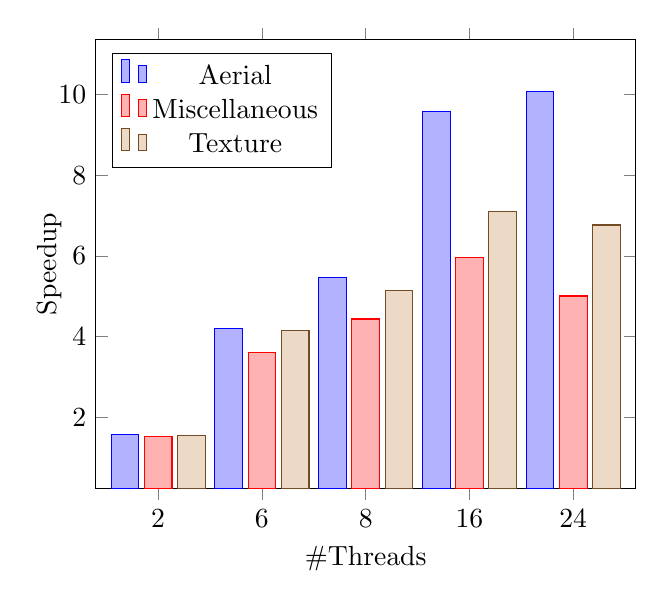
\begin{tikzpicture}
\begin{axis}[
ybar,
enlargelimits=0.15,
legend pos = north west,
xlabel=\#Threads,
ylabel=Speedup,
every axis y label/.style=
{at={(ticklabel cs:0.5)},rotate=90,anchor=center},
symbolic x coords={2,6,8,16,24},
xtick=data,
]
\addplot
coordinates {
(2,1.57)
(6,4.20)
(8,5.46)
(16,9.58)
(24,10.08)

};
\addplot
coordinates {
(2,1.53)
(6,3.60)
(8,4.44)
(16,5.96)
(24,5.01)
};
\addplot
coordinates {
(2,1.56)
(6,4.16)
(8,5.14)
(16,7.10)
(24,6.77)
};

\legend{Aerial,Miscellaneous,Texture}
\end{axis}
\end{tikzpicture}
\caption{Speedup for different images and different numbers of threads for
Aerial, Texture \& Miscellaneous data set}
\label{fig:bar}
\end{figure}


